\newpage
\noindent
\textbf{Beispiel 2}\\ \\
a)\\ \\
Freigeschnittene Platte und Walze:
\begin{figure}[h]
	\centering
	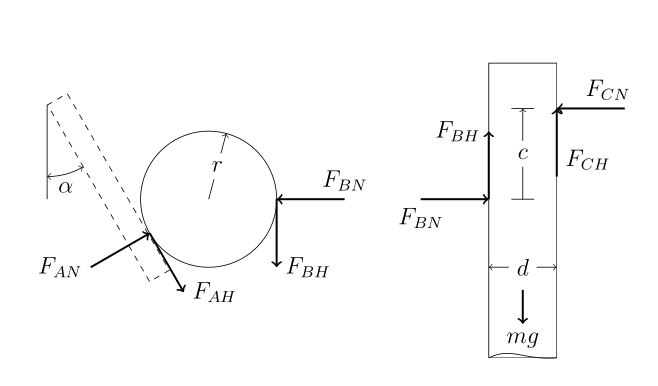
\includegraphics[width= 12.5cm]{tikz/31_03_2017_2a}
\end{figure}
\newline
b)\\ \\
Durch Aufstellen der Kräfte- und Momentenbilanz und mit der Formel für die trockene Haftreibung
\[
	f_C = \mu_Cf_N\text{sign}(\dot{x}) \qquad \text{mit sign}(\dot{x}) = 1
\]
folgt der Reibungskoeffizient
\[
	\mu_W \geq \frac{\sin(\alpha)}{1 + \cos(\alpha)}
\]
c)\\ \\
Durch Aufstellen der Kräfte- und Momentenbilanz  kann die gesuchte Höhe bestimmt werden, die die beiden Momente der Kräfte $F_{CN}$ und $F_{BN}$ ausgleicht. Die Höhe beträgt
\[
	c = \frac{d\sin(\alpha)}{2(1 + \cos(\alpha))}
\]
d)\\ \\
Da die beiden Reibungskoeffizienten nicht vom Gewicht der Platte abhängen, kann die Kraft (bis zur plastischen Verformung) theoretisch unendlich groß sein.